%% amssamp1.tex is nearly identical to amssamp2.tex, except
%% that amssamp2.tex uses the [twocol] option to produce
%% two-column text.

%\documentclass{ametsoc}
\documentclass[twocol]{ametsoc}
\journal{jtech}

%\usepackage{amsmath}
%\usepackage{hyperref}
\usepackage{color}

\usepackage{graphicx}
\graphicspath{{./fig/}}

%%%%%%%%%%%%%%%%%%%%%%%%%%%%%%%%
%Citations should be of the form ``author year''  not ``author, year''
\bibpunct{(}{)}{;}{a}{}{,}

\title{Turbulence spectral estimates from motion-sensor equipped ADVs on compliant moorings}

\authors{Levi Kilcher\correspondingauthor{National Renewable Energy Laboratory, Golden, Colorado}, Jim Thomson, Samuel Harding, and James VanZwieten}

\affiliation{} 

\email{Levi.Kilcher@nrel.gov}

%\extraauthor{Extra Author}
%\extraaffil{Affiliation, City, State/Province, Country}

\graphicspath{{./fig/}}

\newcommand{\note}[1]{\textcolor{blue}{#1}}

\newcommand{\unit}[1]{\ensuremath{\,\mathrm{#1}}}
\def\rmat{\ensuremath{\mathbf{H}}}
%\def\earth{\ensuremath{^\mathrm{e}}}
\def\earth{}
\def\bhv{\ensuremath{\vec{l}_\mathrm{head}^*}}
\def\ihv{\ensuremath{\vec{l}^*_\mathrm{imu}}}
%\def\dolfyn{\url{http://lkilcher.github.io/dolfyn/}{DOLfYN}}
\def\dolfyn{DOLfYN}
\def\omat{\ensuremath{\mathbf{R}}}
\def\omatinv{\ensuremath{\mathbf{R}^\mathrm{T}}}
\def\ue{\ensuremath{\vec{u}\earth}}
\def\uacc{\ensuremath{\ue_a}}

\abstract{
THE ABSTRACT.
}

\begin{document}

\maketitle


\section{Introduction}

% Invented more than twenty years ago, acoustic Doppler velocimeters (ADVs) measure 3-components of velocity by measuring the Doppler shift of an emitted acoustic pulse at 3 

Since their invention more than twenty years ago acoustic Doppler velocimeters (ADVs) have been used to measure turbulent velocities in a wide range of environments. Originally designed to make point-measurements in laboratory flumes and tanks, ADVs have become an increasingly useful tool in the oceanic environment. They have been deployed, for example, on the seafloor to measure fluxes in the oceanic bottom boundary layer, in the surf-zone to measure Reynold's stresses, and from ships on downward protruding masts to measure surface mixing \citep[e.g.]{Lohrmann++1994, Voulgaris+Trowbridge1998, Kim++2000, Trowbridge+Elgar2003, Elgar++2005, Geyer++2008}.

Why is the turbulence spectrum important? -- Captures motion at all scales.
ADCPs 
1) History of ADV use. How are they used? In what turbulence levels? What is their noise-floor? 
1a) How do they compare to other turbulence tools?
Compared to profilers, ADVs are:
  - Lower precision than profilers at high f?
  - Capture low-frequency information.
  - can be fixed in space.
Compared to ADCP, ADVs can capture the turbulence spectrum:
  - Higher precision at high f
  - Higher resolution (down to cm scales)
  - Lower noise

A primary limitation of ADVs is that it has been challenging to place them at mid-depths (i.e. away from the seafloor and the surface). In the oceanic environment they have either been deployed on fixed platforms anchored to the sea-floor, or deployed near the surface from a ship.  Until now, there has been no method for deploying these instruments at mid-water depths, or near the surface without a ship.  This work describes a new approach for measuring turbulence spectra from ADVs mounted on moorings. Until recently this approach has been limited by the fact that mooring motion contaminates the velocity measurements.  The frequency and amplitude of this contamination will depend on the characteristics of the mooring and of the turbulent environment in which it is deployed. In most cases mooring motion will--over some range of frequencies--be similar to or greater than the turbulence velocities one would like to measure. This `motion contamination' reduces usefulness of the ADV measurements. 

Over the last decade, the cost of inertial motion sensors (IMUs)

However, this being said,  In many cases the motion of the mooring Depending Because When the mooring (and ADV head) moves with the flow the measured velocity will be reduced, and when it moves against the flow it will enhance the it. is often equal to the turbulent velocities one would like to measure. contaminates the velocity measurements  equipped with 

In energetic environments ADVs provide 

In energetic environments, where turbulence levels ADVs provide are Throughout 

Velocity measurements have been made from 

As flexible and useful as these instruments are, one limitation 
% boundary-layer studies. 

are useful tools for making point-measurements of water velocity in labarotory and field environments. 
robust and versatile tools 

  ADV velocity measurements from compliant moorings will be contaminated by mooring motion. When an inertial motion unit (IMU, also known as a magnetic, angular rate, gravity or MARG sensor) is rigidly attached to, and tightly synchronized with, acoustic Doppler velocimeter (ADV) measurements the IMU's orientation and motion measurements can be used to reduce motion contamination.  Microstrain IMU on-board the Nortek Vector is equipped with a 3-axis accelerometer, a 3-axis rotation-rate sensor, and a 3-axis magnetometer.  The Microstrain samples these signals at 1000Hz and performs integration and Kalman filtering operations to produce stable estimates of it's orientation, change in velocity, and change in rotation-rate.  and  can be configured to output estimates of,

\section{Measurements}

This work utilizes ADV measurements from two field deployments, and from bench and laboratory tests. The ADVs utilized for these measurements were all equipped with Microstrain 3DM-GX3-25 IMU sensors that captured the angular rotation vector, the linear acceleration, and the orientation of the ADV pressure-case.  

\begin{figure}[t]
  \centering
  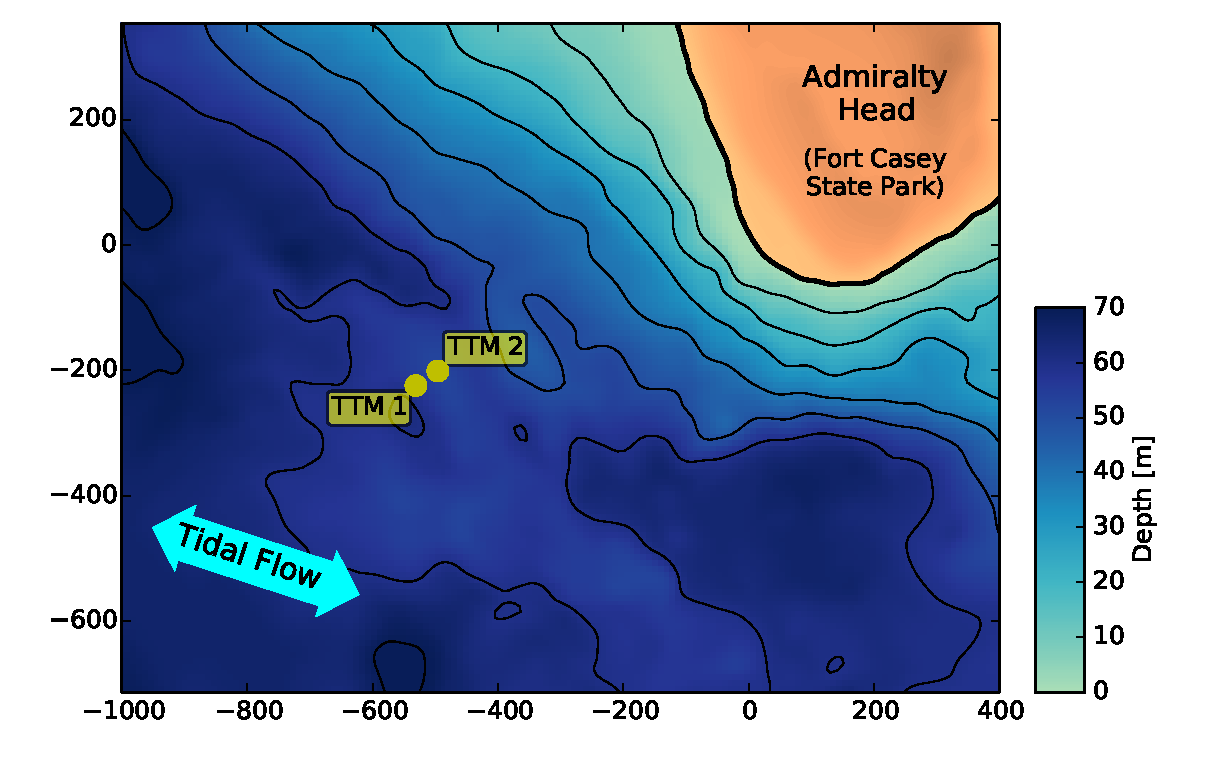
\includegraphics[width=3in]{map02}
  \caption{Map of admiralty inlet.}
  \label{fig:map}
\end{figure}

\begin{figure}[t]
  \centering
  \includegraphics[width=0.8in]{ttm06}
  \caption{TTM schematic.}
  \label{fig:ttm_schematic}
\end{figure}

% Do we need a schematic of the StableMoor too?

\section{Methodology}

Estimate time-series of velocity on a compliant mooring by obtaining an independent estimate of ADV head motion, and removing that motion from the measured signal. Nortek offers an ADV that is equipped with an IMU that measures the linear acceleration and rotational-motion of the ADV pressure case. 
So long as the ADV head is rigidly connected to the ADV pressure case, it is possible to utilize the IMU motion signals to calculate the motion of the ADV head. This motion can then be removed from the measured velocity signal.

A primary limitation of this approach is based on the limitations of the IMU sensors themselves. In particular, the noise levels of the Accel and AngRt signals from the IMU. The primary source of uncertainty in this approach is related to the `low frequency drift' of IMU accelerometers. Without correcting for this, the noise in the Accel will typically overwhelm the measured velocity signal at low frequency, and lead to non-realistic estimates of mean motion (see Appendix \ref{apdx:imu-uncertainty}).

Break motion velocity into two components:
\begin{itemize}
\item translational (Accel + something)
\item rotational  (AngRt)
\end{itemize}

\begin{figure}
  \centering
  
  \caption{Spectra of Accel and AngRt signals, and of the $u_{acc}$ + $u_{rot}$ signals?}
\end{figure}

There are errors in Accel velocity. Discuss these in context of non-moving Accel spectra. Introduce concept of adding low-f translational velocity signal.

\subsection{Motion Correction}\label{sec:proc:motion}

\def\AngRt{\ensuremath{\vec{\omega}}}
\def\Accel{\ensuremath{{\vec{a}^*}}}
\def\Accelp{\ensuremath{{\vec{a}^{*'}}}}
\def\ue{\ensuremath{\vec{u}\earth}}
\def\um{\ensuremath{\ue_\mathrm{h}}}
\def\uadv{\ensuremath{\ue_\mathrm{m}}}
\def\urot{\ensuremath{\ue_\omega}}
\def\uacc{\ensuremath{\ue_a}}

\begin{itemize}
\item the angular rotation rate vector,
\item the linear acceleration vector, and
\item the IMU orientation (matrix), in the earth's 'East-North-Up' (ENU) coordinate system.
\end{itemize}

The orientation matrix can be used to rotate all vector-quantities measured in the instrument frame (velocity, rotation rate, acceleration, etc.) into the earth's coordinate system. 
The angular rate and linear acceleration signals can be used to estimate the ADV head-motion, $\um$, which can then be removed from the measured velocity, $\uadv$, to estimate the `motion corrected' velocity in the earth frame,
\begin{align}
  \label{eqn:u_mot_def}
  \ue(t) & = \uadv(t) + \um(t) &  .
\end{align}
Note that $\um$ is added to $\uadv$ because the measured velocity resulting from head motion is in the opposite direction of head motion itself (i.e., $\uadv = \ue - \um$).


We now break $\um$ into two parts, $ \um  =  \uacc + \urot $.
The first is an estimate of the linear motion of the ADV,
\begin{align}
\label{eqn:uacc-def}
  \uacc(t) & = \int \{\vec{a}\earth(t)\}_{HP(f_{a})} \mathrm{d}t & .
\end{align}
Here, $\vec{a}\earth(t)$ is the IMU-measured acceleration signal rotated into the earth frame\footnote{i.e. $\vec{a}\earth (t) = \omatinv(t) \cdot \vec{a}^*(t)$, see appendix \ref{apdx:coord-sys} for details.}, and $\{\}_{HP(f_{a})}$ denotes an appropriate high pass filter of frequency $f_a$. The acceleration must be high-pass filtered in this way to remove the influence of gravity and that of low-frequency bias drift that is inherent to IMU accelerometer measurements.  

Bench-tests of the Microstrain IMU indicate that its accelerometers drift for frequencies $<10^{-2}$Hz (a minute or more, \cite{EgelandPhD2014}).  Therefore, in order to remove bias-drifts in $\vec{a}$ that--when integrated according to \eqref{eqn:uacc-def}--lead to large errors in $\uacc$ this document recommends using $f_a = 0.033$Hz (30seconds). 
On the other hand, real motions at and below $f_a$ will not be accurately accounted for in $\uacc$, and will therefore persist as low-frequency motion contamination not corrected-for in the estimate of $\vec{u}$. 

For moorings whose low-frequency motion is limited by the mooring line itself this is a reasonable approach.  
Assuming that the displacement of the ADV head (from the mooring's neutral position) is likely to be  $< 20 \% $ of its distance from the bottom, then for ADVs deployed at 10m depth the speed of their low-frequency motion (i.e. below $ f_a = 0.03 $ Hz) will be $<0.07 \mathrm{m/s} $.  In other words, for a 10m mooring the choice of $f_a = 0.03$Hz allows for low-frequency motion contamination on the order of 7cm/s to persist.  This is a notable but relatively minor level of uncertainty in the context of the highly energetic flows that exist at tidal energy sites.

 
The second component if $\um$ is due to rotational motion of the ADV-head about the IMU,
\begin{align}
  \label{eqn:urot-def}
  \urot(t) &  = \omatinv(t) \cdot \left ( \AngRt^*(t)\times\vec{\ell}^*  \right ) & .
\end{align}
Here $\AngRt^*$ is the IMU-measured rotation-rate, $\vec{\ell}^* = \bhv - \ihv$ is the vector from the IMU to the ADV head, $\times$ indicates a cross-product and superscript $*$s denotes a quantity in the `ADV body' coordinate system. This coordinate system is used explicitly here to emphasize that $\vec{\ell}^*$ is constant in time.  Matrix multiplication (denoted by `$\cdot$') with the inverse ADV body orientation matrix, $\omatinv(t)$, is used to rotate the `body-frame rotation induced velocity' into the earth frame.  For details on these coordinate systems and the definition of the orientation matrix see appendix \ref{apdx:coord-sys}.  


\section{Results}

\subsection{Mean velocity}

\begin{figure}[t]
  \centering
  \includegraphics[width=3in]{TimeFig01}
  \caption{Time series of tidal velocity at Admiralty Head.}
  \label{fig:vel_time}
\end{figure}

\subsection{Turbulence Spectra}

Estimates of spectra 

\begin{figure*}[t]
  \centering
  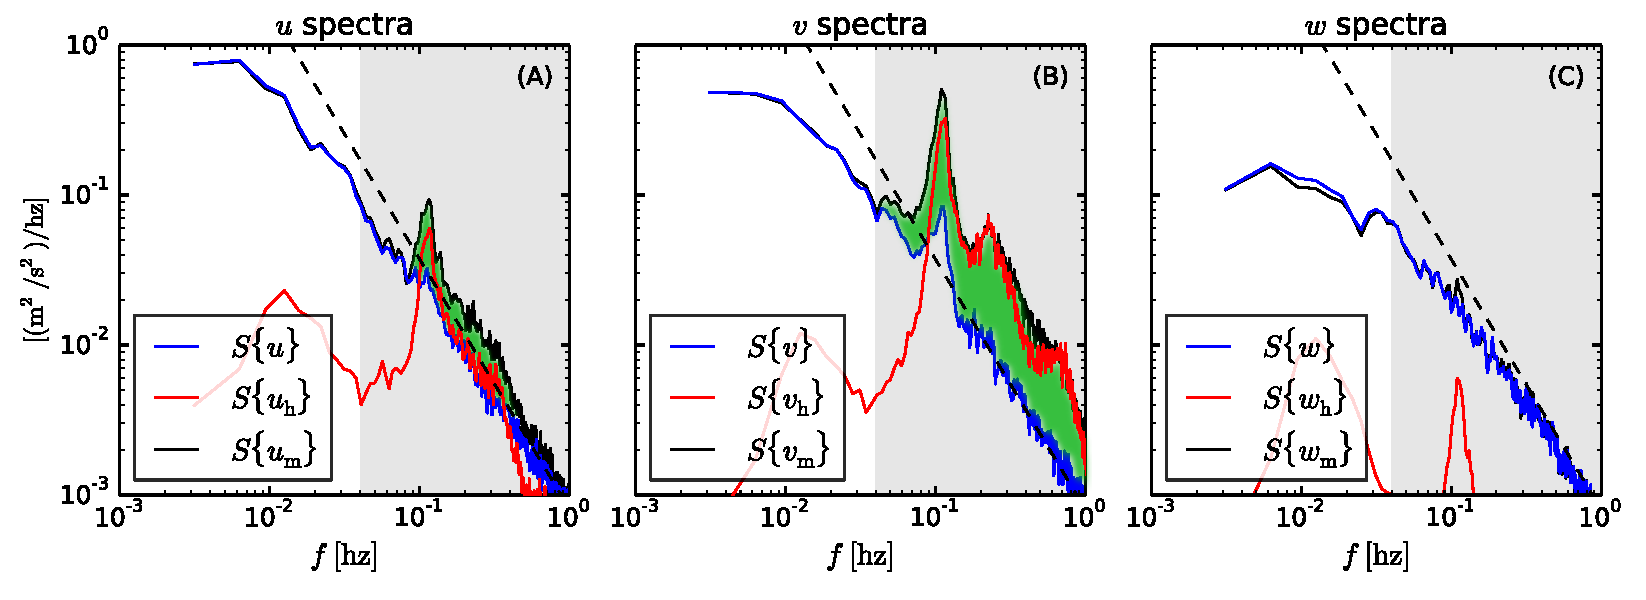
\includegraphics[width=6
in]{SpecFig02_annot}
  \caption{Spectra from IMU-ADV measurements.}
  \label{fig:spec01}
\end{figure*}

\subsubsection{Uncertainty in spectra}

\subsection{Turbulence energy dissipation rate}

%%%%%%%%%%%%%%%%%
%ACKNOWLEDGMENTS
%%%%%%%%%%%%%%%%%

\acknowledgments


\clearpage %REMOVE_FOR_SUBMIT

%%%%%%%%%%%%%%%%%
%APPENDIXES
%%%%%%%%%%%%%%%%%
\appendix

\appendixtitle{Coordinate Systems}

\def\Amat\ensuremath{\mathbf{A}}

\subsection{IMU uncertainty}\label{apdx:imu-uncertainty}

\subsection{Measurement frames}\label{apdx:coord-sys:meas}\label{apdx:coord-sys}

\def\a{\ensuremath{\mathrm{a}}}
\def\b{\ensuremath{\mathrm{b}}}
\def\lab{\ensuremath{l_\b^\a}}
\def\xa{\ensuremath{\vec{r}^\a}}
\def\xb{\ensuremath{\vec{r}^\b}}
\def\Rba{\ensuremath{\mathbf{R}^\a_\b}}

Tracking coordinate systems (`reference frames', or simply `frames') is critical to accurately correcting for platform motion of ADV measurements. In general, two three-dimensional, orthogonal, right-handed coordinate systems `a' and `b' are related by the equation:
\begin{align*}
  \xb &= \Rba \cdot (\xa - \lab) & .
\end{align*}
The vectors $\xa$ and $\xb$ point to the same point in space, but in the two distinct coordinate systems.  Superscripts denote the coordinate system that the quantity is measured in and $\cdot$ indicates standard matrix multiplication.  The vector $\lab$ is the `translation vector' that specifies the origin of coordinate system `b' in the `a' frame, and $\mathbf{R}^\mathrm{a}_\mathrm{b}$ is the `orientation matrix' of `b' in `a'. Note that the equation that maps vectors - as opposed to points in space - from one frame to the other does not include $\lab$:
\begin{align}
  \vec{u}^\mathrm{b} & = \Rba \cdot \vec{u}^\mathrm{a}
\end{align}
Also note that for the orthogonal, right-handed coordinate systems considered here the inverse rotation matrix is simply the transpose, $\mathbf{R}^{\mathrm{b}}_{\mathrm{a}}  = (\Rba)^{-1} = (\Rba)^\mathrm{T} $, and the determinant of the rotation matrix is 1, $\mathrm{det}(\Rba ) = 1$.
The coordinate systems for doing so can be broken into two categories: 1) the `inertial' or `stationary' ones into which it is the goal to transform the measurements, and 2) the moving coordinate systems in which sensors make measurements. 

The purpose of this appendix is to clearly document and define the relationships between all of the coordinate systems necessary for quantifying turbulence using moored ADVs.  This appendix starts with general definitions of coordinate systems and the relationships between them (\ref{apdx:coord-sys:math}), then details the stationary and measurement frames used herein (\ref{apdx:coord-sys:stat} and \ref{apdx:coord-sys:meas}, respectively).

\begin{enumerate}
\item the earth reference frame is the inertial coordinate system in
which it is desirable to have measurements of turbulence velocity
\item the IMU reference frame is the reference frame in which that
sensor measures platform motion
\item the ADV-head reference frame is the reference frame in which the
velocity measurements are obtained.
\end{enumerate}

In addition to measuring platform motion the Microstrain IMU provides
an estimate of the orientation of its coordinate system in the earth's
reference frame. Provided that the position and orientation of the
ADV-head is known and fixed in the IMU frame (i.e. they are rigidly
connected), it is possible to estimate the motion of the ADV-head in
the earth reference frame.




\subsection{Defining coordinate systems}\label{apdx:coord-sys:math}


\subsection{The earth frame}
The earth coordinate system is the coordinate system in-which the orientation of the ADV is measured (see \ref{apdx:coord-sys:imu}), and is the coordinate system in-which motion correction is most easily calculated and discussed (section \ref{sec:proc:motion}).  This work utilizes `e' superscripts to denote an `ENU' earth coordinate system with basis vectors,
\begin{itemize}
\item[$\hat{x}\earth$:] East,
\item[$\hat{y}\earth$:] North, and
\item[$\hat{z}\earth$:] Up.
\end{itemize}

\begin{figure*}
  \centering
  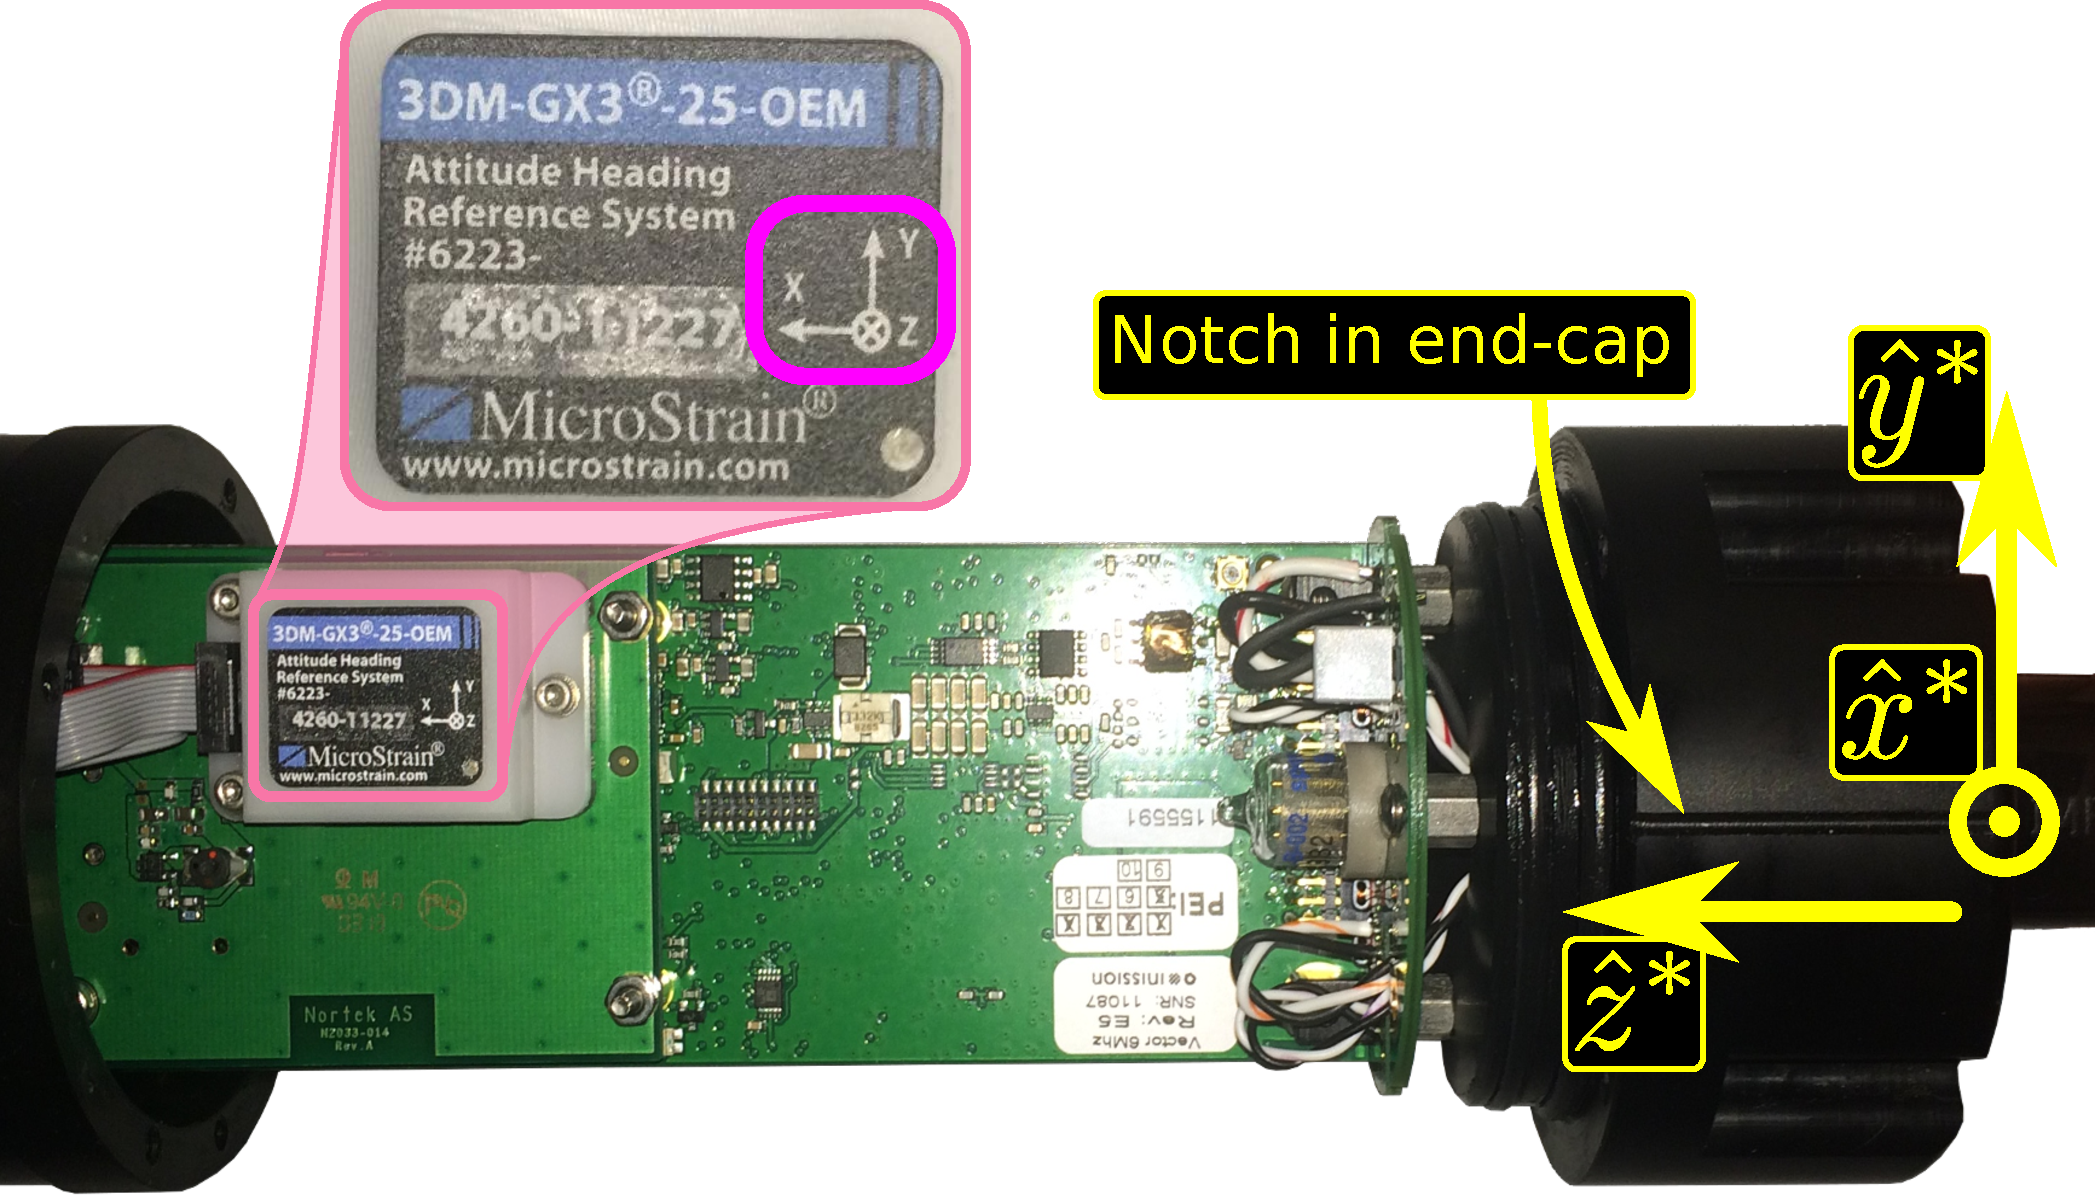
\includegraphics[width=4in]{IMUtest}
  \caption{The circuit-board and pressure-case end-cap of a Nortek Vector equipped with a Microstrain IMU.  The ADV-body coordinate system (yellow) is depicted on the right. The notch in the end-cap defines the $\hat{x}^*$ direction (out of the page), and the $\hat{z}^*$ direction points back along the pressure case axis. A zoom-in on the Microstrain chip highlights its coordinate system (magenta) relative to the body. }
  \label{fig:imu_orient}
\end{figure*}

To combine signals from an IMU with those of an ADV to perform motion correction the coordinate systems in which each of the measurements are made must be carefully accounted for. 

For the Nortek Vector instruments that were used for this work the `ADV-body' coordinate system is defined as being centered on the cylinder-body axis at the point where the head-cable meets its end-cap.  The basis vectors of this coordinate system are defined as (Figures \ref{fig:imu_orient} and \ref{fig:adv-coord-sys}B):
\begin{itemize}
\item[$\hat{x}^*$:] points from the center of the `head' end-cap toward the notch in that end-cap,
\item[$\hat{y}^*$:] is defined by the right-hand-rule based on the other two basis vectors, and
\item[$\hat{z}^*$:] points from the `head' end-cap toward the `battery' end-cap along the body-cylinder (pressure case) axis.
\end{itemize}

\subsubsection{The ADV head}

In order to transform measured velocities into a meaningful reference frame (and to perform motion correction) the orientation (and position) of the ADV head in terms of the body coordinate system must be known. To facilitate this the orientation matrix of the ADV head, $\rmat$, and translation vector\footnote{The position of the ADV-head origin (transmit transducer) in the body coordinate system.}, $\bhv$, are defined according to,
\begin{align}
  \label{eqn:coord_sys}
  \vec{x}^\mathrm{head} &= \rmat \cdot (\vec{x}^* - \bhv) & ,
\end{align}
where $\vec{x}^\mathrm{head}$ and $\vec{x}^*$ are the same point in the head and body coordinate systems, respectively. Combined with the math notes in the previous section, the velocity vectors in the head frame can be transformed into the body frame by,
\begin{align}
  \label{eqn:coord_sys2}
  \vec{u}^* &=  \rmat^\mathrm{T} \cdot \vec{u}^\mathrm{head} & .
\end{align}

For Nortek Vectors, the coordinate system of the ADV head is centered on the transmit transducer face, and the coordinate-directions are defined by (Figure \ref{fig:adv-coord-sys}B, \cite{vector_manual2005}):
\begin{itemize}
\item[$\hat{x}^\mathrm{head}$:] the direction of one of the transducer `receive' arms (marked with tape or paint)
\item[$\hat{y}^\mathrm{head}$:] is defined by the right-hand-rule based on the other two basis vectors, and
\item[$\hat{z}^\mathrm{head}$:] is into the transducer face.
\end{itemize}

For fixed-head Nortek Vector ADVs, the body-frame and head-frame have parallel coordinate systems ($\rmat$ is the identity matrix), and the `head-frame' is translated 21cm along the $z$-axis.  That is, $\bhv = (0, 0, -0.21)$m \cite[]{vector_manual2005}.  

For cable-head ADVs, the position and orientation of the ADV head is arbitrary.  This means that when preparing to make measurements using cable-head ADVs, {\bf the orientation and position of the ADV head must be accurately recorded} in order to allow the ADV measurements to be transformed into the body frame during post-processing. For the example in Figure \ref{fig:adv-coord-sys}A, $\bhv = (254,64,-165)\unit{mm}$, and
\begin{align*}
  \rmat &= \left (
    \begin{array}{ccc}
      0 & 0 & -1 \\
      0 & -1 & 0 \\
      -1 & 0 & 0
    \end{array}
    \right ) & .
\end{align*}
In general $\rmat$ will not necessarily be symmetric nor will it have so many zero-elements (i.e. these characteristics are specific to the head-body alignment of the example).


\begin{figure*}
  \centering
    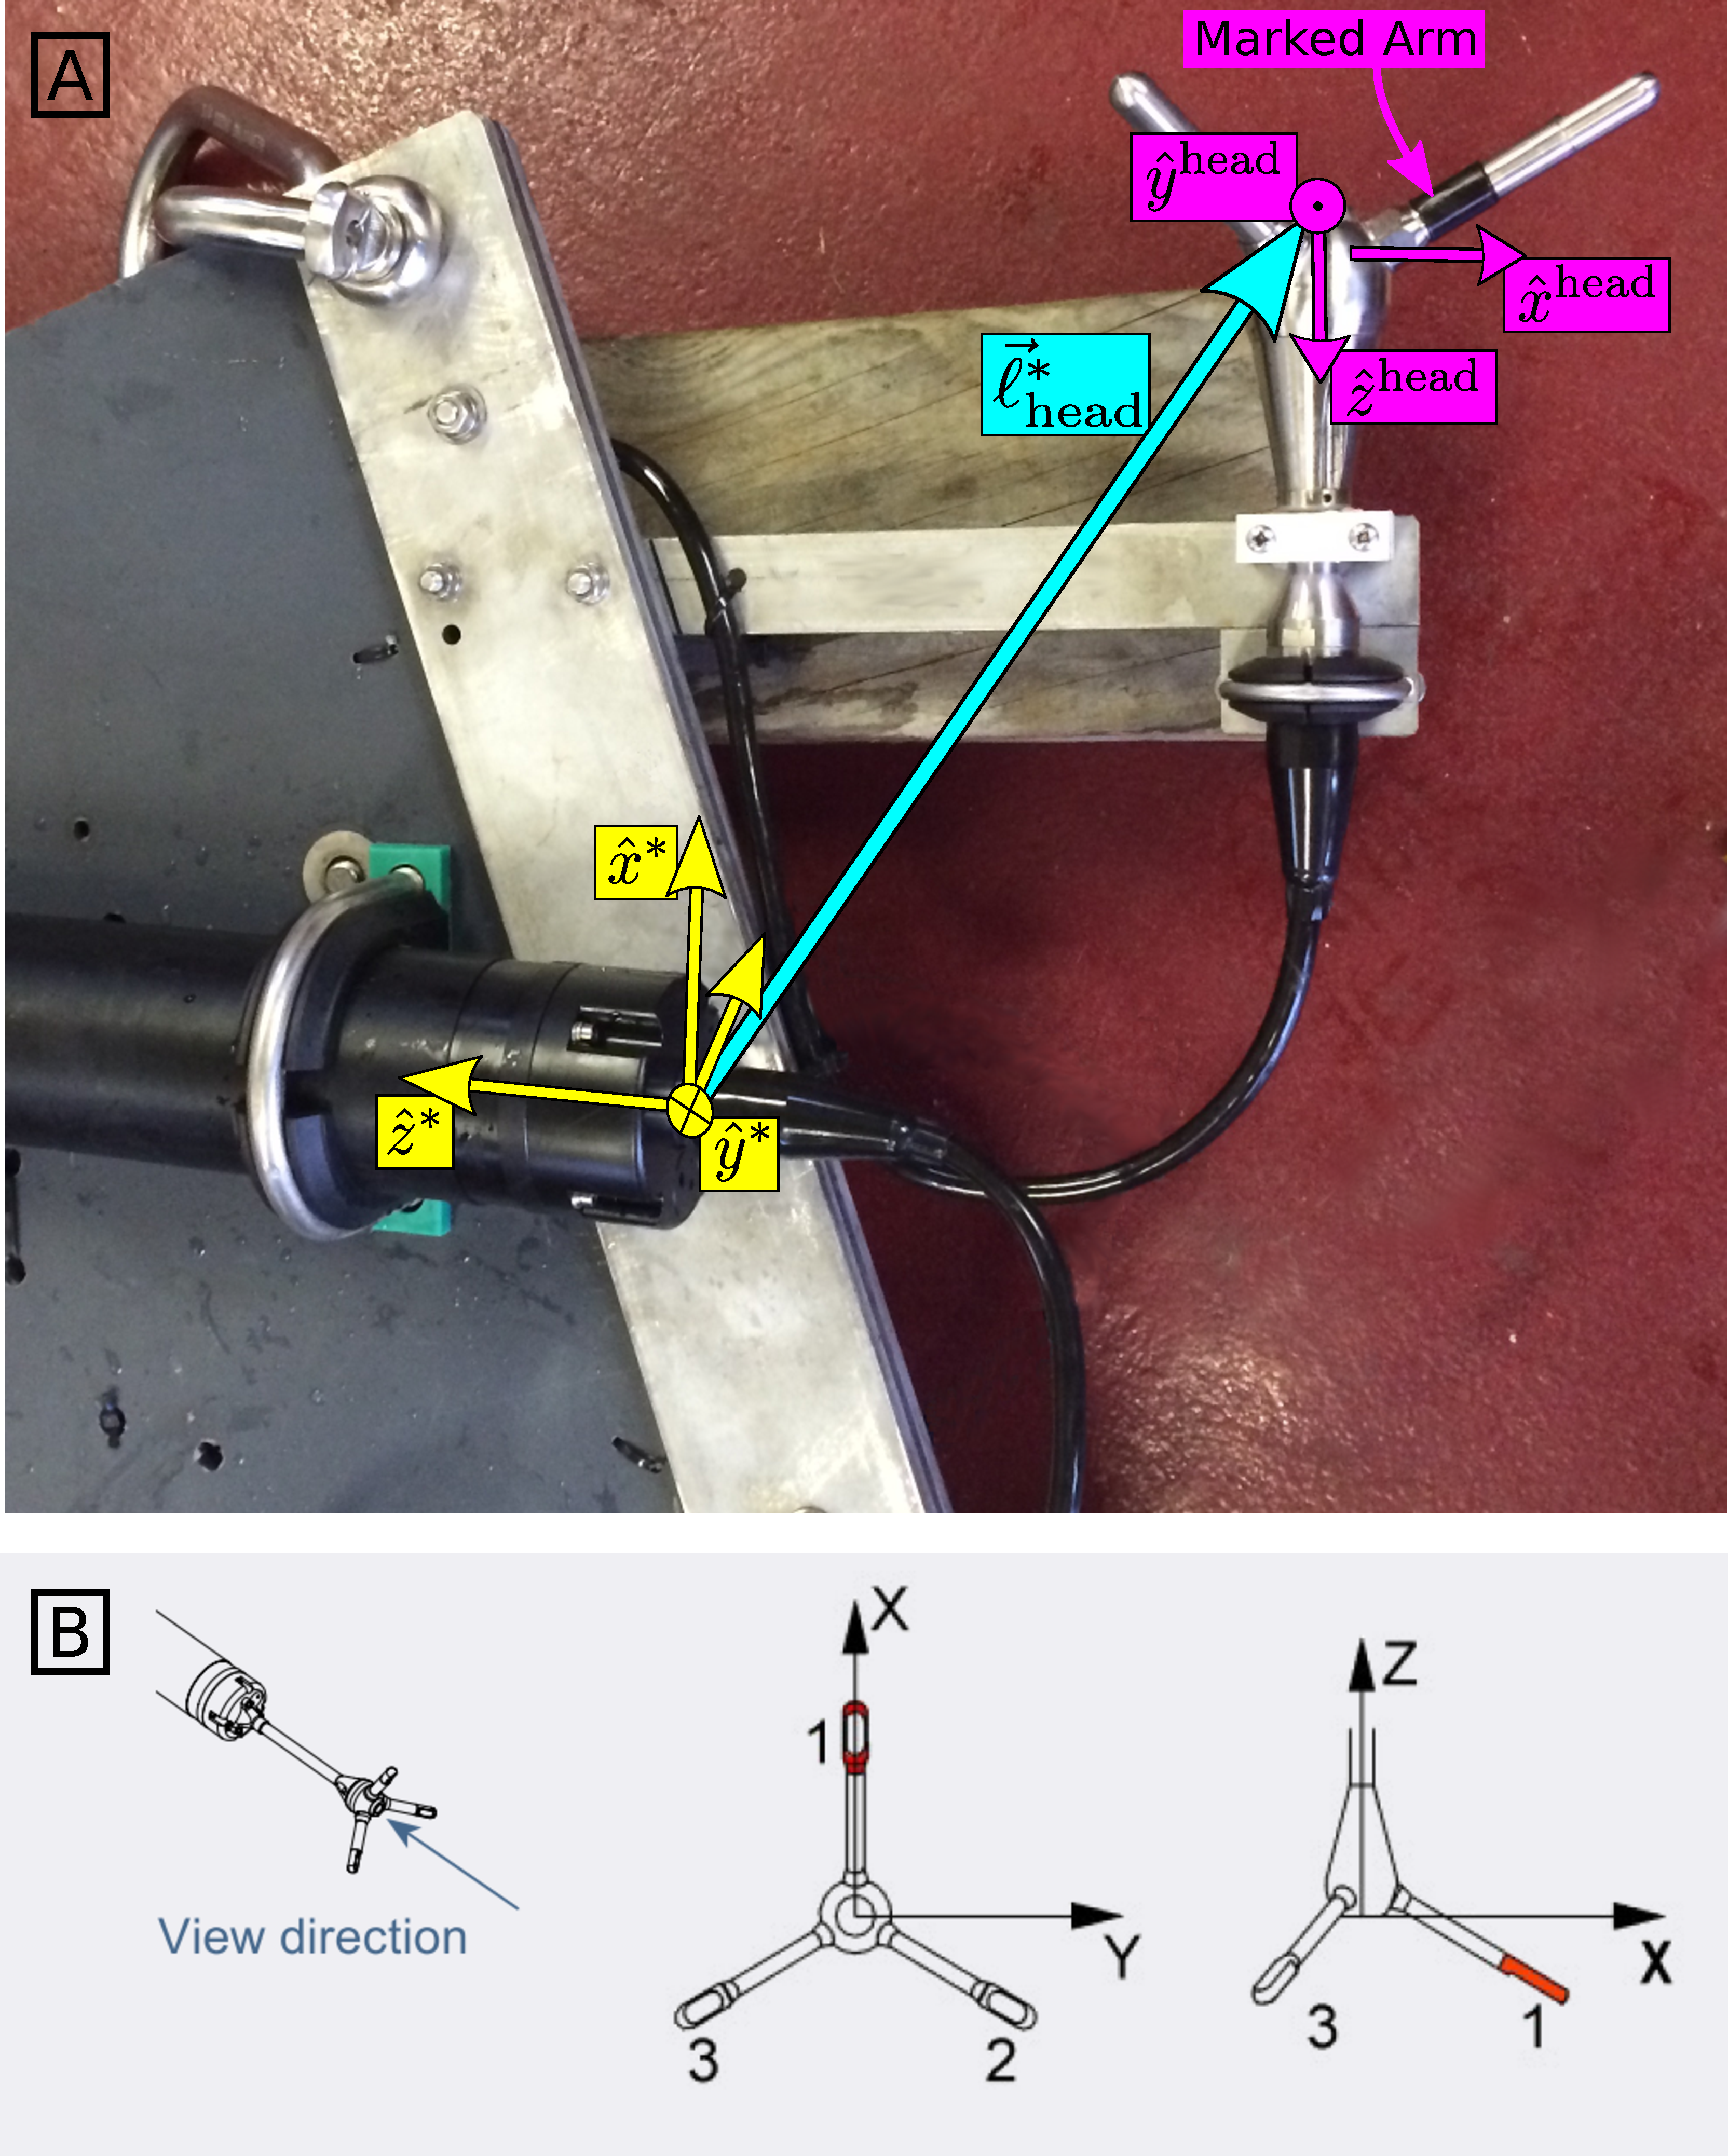
\includegraphics[width=4in]{ADV_coord_sys4}
  \caption{Coordinate systems of the ADV body and head. A) A strongback with an ADV rests on a block of wood. Coordinate systems of the ADV head (magenta) and body (yellow) are shown. The $\hat{x}^\mathrm{head}$-direction is known by the black-band around the transducer arm, and the $\hat{x}^*$ direction is marked by a notch on the end-cap (indiscernible in the image). The cyan arrow indicates the body-to-head vector, $\bhv$.  The perspective slightly distorts the fact that  $\hat{x}^\mathrm{head} \parallel -\hat{z}^* $, $\hat{y}^\mathrm{head} \parallel -\hat{y}^* $, and $\hat{z}^\mathrm{head} \parallel -\hat{x}^* $.  B) Coordinate system of the ADV head as defined in the Nortek Vector manual \cite[]{vector_manual2005}. }
  \label{fig:adv-coord-sys}
\end{figure*}

\subsubsection{The IMU coordinate system}\label{apdx:coord-sys:imu}

Like the ADV head, the coordinate system in which the IMU measurements are made must be clearly defined and documented. In general, the IMU frame is related to the body coordinate system by,
\begin{align*}
  \vec{x}^\mathrm{imu} &= \mathbf{A}  \cdot (\vec{x}^* - \ihv) & \qquad .
\end{align*}

For the Microstrain 3DM-GX3-25 (IMU) as it is integrated into the Nortek Vector (Figure \ref{fig:imu_orient}), $\ihv = (0.006, 0.006, 0.150)$m and,
\begin{align*}
  \mathbf{A} &=
  \left (
    \begin{array}{ccc}
      0 & 0 & 1 \\
      0 & 1 & 0 \\
      -1 & 0 & 0
    \end{array}
  \right ) & .
\end{align*}


{\bf The orientation matrix}
\def\omatr{\ensuremath{\mathrm{\mathbf{R_\mathrm{imu}}}}}

In order to use the orientation matrix to rotate velocity measurements into an earth-fixed coordinate system it is important to understand how the orientation matrix is defined. The Microstrain IMU outputs an orientation matrix, \omatr, such that:
\begin{align*}
  \vec{u}^\mathrm{imu} & = \omatr \cdot \vec{u}^\mathrm{NED} & .
\end{align*}
Where $\vec{u}^\mathrm{imu}$ and $\vec{u}^\mathrm{NED}$ are vectors in the IMU's local coordinate system and a `north-east-down' (NED) earth-fixed coordinate system, respectively \cite[]{Microstrain2012a}.  
However, this NED earth coordinate system is different from the ENU earth coordinate system used here (and typically used by Nortek \cite[]{nortek_sys_int_manual2011}).  That is,
\begin{align*}
  \vec{u} &= \mathbf{B} \cdot \vec{u}^\mathrm{NED} & ,
\end{align*}
where,
\begin{align*}
  \mathbf{B} & = 
  \left (
    \begin{array}{ccc}
      0 & 1 & 0 \\
      1 & 0 & 0 \\
      0 & 0 & -1
    \end{array}
  \right ) \qquad .
\end{align*}
From this, and the above discussion of the orientation of the IMU in the ADV, it is simple to show that the orientation matrix of the ADV body in a ENU earth frame is,
\begin{align*}
  \omat &= \mathbf{A} \cdot \omatr \cdot \mathbf{B} & ,
\end{align*}
%The \dolfyn\ software package makes this transformation when reading the orientation matrix from Nortek Vector `{\it .vec}' files (i.e. the `orientmat' attribute in the data object returned by \dolfyn .io.read\_nortek is \omat, not \omatr ).  This way vectors in the body frame can be rotated into the ENU earth frame by,
 % \begin{align*}
 %   \vec{u} & = \omatinv \cdot \vec{u}^* & .
 % \end{align*}


%%%%%%%%%%%%%%%%%
%REFERENCES
%%%%%%%%%%%%%%%%%

\bibliographystyle{ametsoc2014}
\bibliography{all}


\end{document}





